\chapter{ऐरोमैटिकता और इलेक्ट्रॉनरागी ऐरोमैटिक प्रतिस्थापन}\label{ch:b2:aromatic-substitution}

ब्रोमीन जल किसी ऐल्कीन के साथ हिलाने पर कुछ ही सेकंडों में रंगहीन हो जाता है,
और बेन्ज़ीन के साथ बिल्कुल नहीं। फिर भी थोड़ा आयरन(III) ब्रोमाइड मिलाते ही बेन्ज़ीन
ब्रोमीन से अभिक्रिया करती है --- और उत्पाद, ब्रोमोबेन्ज़ीन, का षट्सदस्यी \omterm{def:b2:huckel:aromatic}{ऐरोमैटिक} वलय
बना रहता है: एक हाइड्रोजन प्रतिस्थापित हुआ है, कुछ भी जोड़ा नहीं गया।
\omterm{def:b2:huckel:aromatic}{ऐरोमैटिक} वलय योग के बजाय प्रतिस्थापन करते हैं, क्योंकि योग
\cref{ch:b2:huckel} में परिकलित स्थायीकरण को गँवा देता। वही
क्रियाविधि बेन्ज़ीन वलयों का नाइट्रीकरण, सल्फ़ोनीकरण, ऐल्किलन और ऐसिलन करती है, और
वलय पर पहले से स्थित समूह, आश्चर्यजनक नियमितता के साथ, तय करते हैं कि
अगला समूह कहाँ जाएगा।

\begin{recall}
\Cref{ch:b2:huckel}: ऐरोमैटिकता और बेन्ज़ीन की \omterm{def:b2:huckel:delocalisation}{विस्थानीकरण ऊर्जा}। प्रथम वर्ष का
खंड: ऐल्कीनों पर इलेक्ट्रॉनरागी योग, प्रेरणिक और मेसोमेरी प्रभाव, दाता और
ग्राही समूह, कार्बधनायन और उनके पुनर्विन्यास, हैमंड अभिगृहीत, लुइस अम्ल,
ऊर्जा आरेख।
\end{recall}

\begin{omfigure}
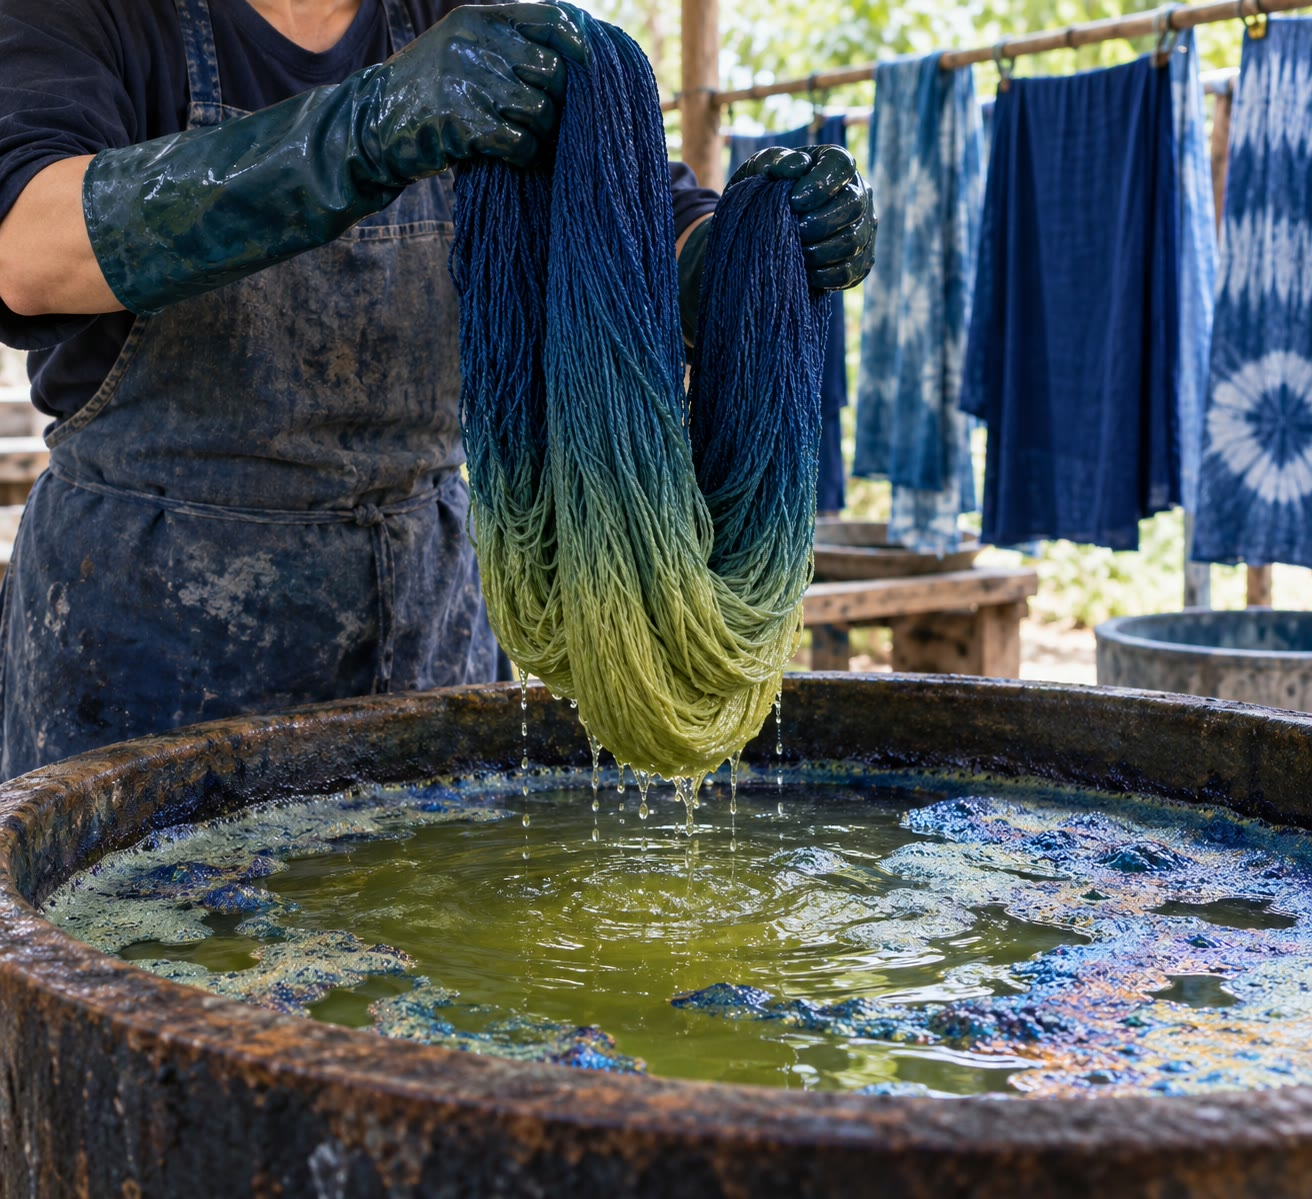
\includegraphics[width=0.55\linewidth]{images/book3/ai/b2-22-indigo-vat-2.jpg}

{\small नील के कुंड में सूत की रँगाई (चित्रण)। सूत कुंड से पीला-हरा निकलता है, रंजक के
विलेय अपचित रूप से भीगा हुआ, और वायु में नीला हो जाता है जब ऑक्सीजन उसे फिर
अविलेय नील में बदल देती है। अधिकांश रंजकों की तरह नील \omterm{def:b2:huckel:aromatic}{ऐरोमैटिक} वलयों पर बना है;
उन्नीसवीं शताब्दी का रंजक उद्योग कोलतार से प्राप्त बेन्ज़ीन पर लागू
इस अध्याय की प्रतिस्थापन अभिक्रियाओं से विकसित हुआ।}
\end{omfigure}

\section{प्रतिस्थापन, योग नहीं}

\begin{definition}[ऐरीन]\label{def:b2:aromatic-substitution:arene}
\emph{ऐरीन}\index{ऐरीन} वह हाइड्रोकार्बन है जिसमें कम-से-कम एक \omterm{def:b2:huckel:aromatic}{ऐरोमैटिक} वलय हो, जैसे
बेन्ज़ीन, टॉलूईन (मेथिलबेन्ज़ीन) या नैफ़्थलीन; ऐरिल समूह (\ce{Ar}) एक हाइड्रोजन कम
ऐरीन है।
\end{definition}

\begin{proposition}[बेन्ज़ीन योग क्यों नहीं करती]\label{prop:b2:aromatic-substitution:no-addition}
बेन्ज़ीन पर योग \omterm{def:b2:huckel:aromatic}{ऐरोमैटिक} वलय को अनैरोमैटिक साइक्लोहेक्साडाईन में बदल देता और
\omterm{def:b2:huckel:aromatic}{ऐरोमैटिक} स्थायीकरण के \qty{150}{kJ/mol} का अधिकांश भाग गँवा देता; प्रतिस्थापन उसे बनाए रखता है।
\end{proposition}

\begin{proof}[तर्क]
\cref{ch:b2:huckel} में बेन्ज़ीन का साइक्लोहेक्सा-1,3-डाईन में हाइड्रोजनन
\omterm{def:b2:reaction-enthalpy:exothermic}{ऊष्माशोषी} पाया गया (\qty{+22}{kJ/mol}, \qty{-206.0}{} और \qty{-227.7}{kJ/mol} से), जबकि
किसी सामान्य द्वि-आबंध का हाइड्रोजनन \qty{119}{kJ/mol} मुक्त करता है: पहला योग महँगा चरण है।
पहले इलेक्ट्रॉनरागी चरण के बाद बना धनायन या तो कोई नाभिकरागी जोड़ सकता है, जो
एक अनैरोमैटिक \omterm{def:b2:frontier-orbitals:diels-alder}{डाईन} छोड़ता है, या एक प्रोटॉन खो सकता है, जो \omterm{def:b2:huckel:aromatic}{ऐरोमैटिक} वलय को पुनः स्थापित करता है। दूसरा
पथ कहीं अधिक अनुकूल है।
% ledger: dfh:C6H6_g, dfh:C6H8_g, dfh:C6H10_g, dfh:C6H12_g
\end{proof}

\section{क्रियाविधि}

\begin{definition}[इलेक्ट्रॉनरागी ऐरोमैटिक प्रतिस्थापन]\label{def:b2:aromatic-substitution:seAr}
\emph{इलेक्ट्रॉनरागी ऐरोमैटिक प्रतिस्थापन}\index{इलेक्ट्रॉनरागी ऐरोमैटिक प्रतिस्थापन}
किसी \omterm{def:b2:huckel:aromatic}{ऐरोमैटिक} वलय के एक हाइड्रोजन को इलेक्ट्रॉनरागी \ce{E+} से प्रतिस्थापित करता है। इलेक्ट्रॉनरागी पहले
वलय के एक कार्बन से आबंधित होता है, जिससे ऐसा धनायन बनता है जिसमें वह कार्बन चतुष्फलकीय है और
धनात्मक आवेश शेष पाँच पर फैला है: \emph{व्हीलैंड मध्यवर्ती}\index{व्हीलैंड मध्यवर्ती}
(एक ऐरीनियम आयन)। फिर कोई क्षारक चतुष्फलकीय कार्बन से प्रोटॉन हटाता है।
\end{definition}

\begin{proposition}[दो चरण]\label{prop:b2:aromatic-substitution:mechanism}
पहला चरण, जो ऐरोमैटिकता को नष्ट करता है, धीमा है; प्रोटॉन का निष्कासन,
जो उसे पुनः स्थापित करता है, तेज़ है।
\end{proposition}

\begin{proof}[तर्क]
\omterm{def:b2:aromatic-substitution:seAr}{व्हीलैंड मध्यवर्ती} तीन कार्बनों पर विस्थानीकरण से स्थायीकृत एक कार्बधनायन है
परंतु \omterm{def:b2:huckel:aromatic}{ऐरोमैटिक} नहीं: वह अभिकारकों से बहुत ऊपर है, और हैमंड अभिगृहीत के अनुसार
उस तक ले जाने वाली संक्रमण अवस्था संरचना और ऊर्जा में उसके निकट है। दूसरा चरण
नीचे एक \omterm{def:b2:huckel:aromatic}{ऐरोमैटिक} उत्पाद तक ले जाता है: उसका अवरोध नीचा है।
\end{proof}

\begin{omfigure}
\begin{tikzpicture}
\begin{axis}[width=0.55\linewidth, height=5.4cm, xmin=-0.2, xmax=4.2, ymin=-5.5, ymax=11.5,
  axis x line=bottom, axis y line=left, xtick=\empty, ytick=\empty,
  xlabel={अभिक्रिया निर्देशांक}, ylabel={ऊर्जा}, label style={font=\small}, clip=false]
\addplot[omDef, thick] table[x=x, y=sub] {figdata/out/bachelor-2-aromatic-profile.dat};
\addplot[omThm, thick, dashed, restrict x to domain=2:4] table[x=x, y=add] {figdata/out/bachelor-2-aromatic-profile.dat};
\node[font=\scriptsize, anchor=north west] at (axis cs:0.0,-0.6) {\ce{ArH + E+}};
\node[font=\scriptsize, anchor=north] at (axis cs:2,5.7) {व्हीलैंड};
\node[font=\scriptsize, anchor=west, omDef] at (axis cs:4.05,-4.0) {\ce{ArE + H+}};
\node[font=\scriptsize, anchor=west, omThm] at (axis cs:4.05,2.0) {योग उत्पाद};
\node[font=\scriptsize, anchor=south] at (axis cs:1,10.1) {धीमा};
\end{axis}
\end{tikzpicture}

{\small किसी \omterm{def:b2:aromatic-substitution:seAr}{इलेक्ट्रॉनरागी ऐरोमैटिक प्रतिस्थापन} का ऊर्जा आरेख, व्यवस्था-रूप (एक मॉडल)।
पहले चरण का, जो \omterm{def:b2:aromatic-substitution:seAr}{व्हीलैंड मध्यवर्ती} बनाता है, अवरोध सबसे ऊँचा है। प्रोटॉन का
निष्कासन (ठोस) \omterm{def:b2:huckel:aromatic}{ऐरोमैटिक} वलय को पुनः स्थापित करता है; किसी नाभिकरागी का योग (खंडित) अभिकारकों से
ऊपर का उत्पाद छोड़ता।}
\end{omfigure}

\begin{omfigure}
\setchemfig{atom sep=2em}
\schemestart
\chemfig{HO-\chemabove{N}{\scriptstyle +}(=[1]O)-[7]\chemabove{O}{\scriptstyle -}} \+ \chemfig{H_2SO_4}
\arrow{<=>}
\chemfig{O=N^{+}=O} \+ \chemfig{HSO_4^{-}} \+ \chemfig{H_2O}
\schemestop

\medskip
\begin{tikzpicture}[font=\small, >={Stealth}]
\tikzset{pics/whel/.style n args={4}{code={
    \foreach \k in {0,...,5} \draw[thick] ({90+60*\k}:0.7) -- ({150+60*\k}:0.7);
    \foreach \k in {#1} \draw[thick] ($({90+60*\k}:0.56)!0.18!({150+60*\k}:0.56)$) -- ($({90+60*\k}:0.56)!0.82!({150+60*\k}:0.56)$);
    \ifnum#2>-1 \node[font=\scriptsize] at ({90+60*#2}:0.36) {$+$};\fi
    \draw[thick] (270:0.7) -- ++(-125:0.42) node[anchor=north east, inner sep=1pt, font=\scriptsize] {H};
    \draw[thick] (270:0.7) -- ++(-55:0.42) node[anchor=north west, inner sep=1pt, font=\scriptsize] {#4};
    \if\relax\detokenize{#3}\relax\else
      \draw[thick] (90:0.7) -- (90:1.1) node[anchor=south, inner sep=1pt, font=\scriptsize] {#3};\fi
  }}}
  \foreach \k in {0,...,5} \draw[thick] ({90+60*\k}:0.7) -- ({150+60*\k}:0.7);
  \foreach \k in {0,2,4} \draw[thick] ($({90+60*\k}:0.56)!0.18!({150+60*\k}:0.56)$) -- ($({90+60*\k}:0.56)!0.82!({150+60*\k}:0.56)$);
  \node at (1.3,0) {$+$};
  \node at (2.0,0) {\ce{NO2+}};
  \draw[->, thick] (2.6,0) -- (3.8,0) node[midway, above, font=\scriptsize] {धीमा};
  \pic at (4.7,0.1) {whel={1,4}{0}{}{\ce{NO2}}};
  \draw[->, thick] (5.6,0) -- (6.8,0) node[midway, above, font=\scriptsize] {तेज़} node[midway, below, font=\scriptsize] {$-$\ce{H+}};
  \begin{scope}[xshift=7.7cm]
    \foreach \k in {0,...,5} \draw[thick] ({90+60*\k}:0.7) -- ({150+60*\k}:0.7);
    \foreach \k in {0,2,4} \draw[thick] ($({90+60*\k}:0.56)!0.18!({150+60*\k}:0.56)$) -- ($({90+60*\k}:0.56)!0.82!({150+60*\k}:0.56)$);
    \draw[thick] (270:0.7) -- (270:1.1) node[anchor=north, font=\scriptsize] {\ce{NO2}};
  \end{scope}
\end{tikzpicture}
\par\vspace{6pt}

{\small बेन्ज़ीन का नाइट्रीकरण। सल्फ़्यूरिक अम्ल नाइट्रिक अम्ल को प्रोटॉनित करता है, जो जल खो देता है:
नाइट्रोनियम आयन \ce{NO2+} इलेक्ट्रॉनरागी है। यह एक कार्बन से आबंधित होता है (धीमा), जिससे
\omterm{def:b2:aromatic-substitution:seAr}{व्हीलैंड मध्यवर्ती} बनता है, जिसका धनात्मक आवेश वलय पर फैला होता है; प्रोटॉन का निष्कासन
(तेज़) नाइट्रोबेन्ज़ीन देता है।}
\end{omfigure}

\section{अभिक्रियाएँ}

\paragraph{हैलोजनन।} केवल ब्रोमीन या क्लोरीन बहुत दुर्बल इलेक्ट्रॉनरागी है; कोई लुइस अम्ल
(\ce{FeBr3}, \ce{AlCl3}) हैलोजन के एक परमाणु से बँधकर उसे ध्रुवित करता है, और बाहरी
ब्रोमीन वलय पर आक्रमण करता है।

\paragraph{नाइट्रीकरण।} सांद्र नाइट्रिक और सल्फ़्यूरिक अम्लों का मिश्रण (ऊपर)
नाइट्रोनियम आयन देता है।

\paragraph{सल्फ़ोनीकरण।} धूमायमान सल्फ़्यूरिक अम्ल (\ce{SO3} में \ce{H2SO4}) बेन्ज़ीनसल्फ़ोनिक अम्ल देता है।
अभिक्रिया उत्क्रमणीय है: सल्फ़ोनिक अम्ल को तनु जलीय अम्ल में गर्म करने से
\ce{SO3H} समूह फिर हट जाता है, जो इसे एक उपयोगी अस्थायी अवरोधक समूह बनाता है।

\begin{definition}[फ़्रीडेल--क्राफ़्ट्स अभिक्रियाएँ]\label{def:b2:aromatic-substitution:friedel-crafts}
\emph{फ़्रीडेल--क्राफ़्ट्स ऐल्किलन}\index{फ़्रीडेल--क्राफ़्ट्स ऐल्किलन} किसी हैलोऐल्केन और
किसी लुइस अम्ल (\ce{AlCl3}) से किसी \omterm{def:b2:huckel:aromatic}{ऐरोमैटिक} वलय पर एक ऐल्किल समूह जोड़ता है।
\emph{फ़्रीडेल--क्राफ़्ट्स ऐसिलन}\index{फ़्रीडेल--क्राफ़्ट्स ऐसिलन} एक ऐसिल समूह
\ce{RCO} जोड़ता है, किसी ऐसिल क्लोराइड और \ce{AlCl3} से, \emph{ऐसिलियम आयन}\index{ऐसिलियम आयन}
\ce{R-C#O+} के माध्यम से, और एक ऐरिल कीटोन देता है।
\end{definition}

\begin{proposition}[फ़्रीडेल--क्राफ़्ट्स अभिक्रियाओं की सीमाएँ]\label{prop:b2:aromatic-substitution:friedel-crafts-limits}
\omterm{def:b2:aromatic-substitution:friedel-crafts}{फ़्रीडेल--क्राफ़्ट्स ऐल्किलन} कार्बधनायन के पुनर्विन्यासों और
बहु-ऐल्किलन से ग्रस्त है; ऐसिलन एक प्रतिस्थापन के बाद रुक जाता है, कोई पुनर्विन्यास नहीं देता, और उसे कम-से-कम
\ce{AlCl3} का एक तुल्यांक चाहिए। प्रबल \omterm{def:b2:aromatic-substitution:directing}{निष्क्रियक समूह} वाले वलय पर दोनों में से कोई भी
काम नहीं करता।
\end{proposition}

\begin{proof}[तर्क]
ऐल्किलन करने वाला इलेक्ट्रॉनरागी एक कार्बधनायन है (या एक ध्रुवित संकुल जो उसकी तरह व्यवहार करता है),
जो हाइड्राइड या ऐल्किल विस्थापन द्वारा अधिक स्थायी कार्बधनायन में पुनर्विन्यस्त होता है: 1-क्लोरोप्रोपेन
अधिकांशतः आइसोप्रोपिलबेन्ज़ीन देता है। ऐल्किल समूह वलय को सक्रिय करता है (अगला खंड), अतः उत्पाद
बेन्ज़ीन से तेज़ अभिक्रिया करता है और फिर से ऐल्किलित होता है। \omterm{def:b2:aromatic-substitution:friedel-crafts}{ऐसिलियम आयन}
अनुनाद से स्थायीकृत है (\ce{R-C+=O} $\leftrightarrow$ \ce{R-C#O+}) और पुनर्विन्यस्त नहीं होता; ऐसिल समूह
वलय को निष्क्रिय करता है, अतः उत्पाद आगे अभिक्रिया नहीं करता; और बना कीटोन अपने ऑक्सीजन से
\ce{AlCl3} को बाँध लेता है, उत्प्रेरक को अभिक्रिया से हटाते हुए: एक तुल्यांक
उपभुक्त होता है। प्रबल रूप से निष्क्रियित वलय इन दुर्बल इलेक्ट्रॉनरागियों के लिए बहुत क्षीण नाभिकरागी है।
\end{proof}

\section{प्रतिस्थापी प्रभाव}

\begin{definition}[निर्देशक समूह]\label{def:b2:aromatic-substitution:directing}
बेन्ज़ीन वलय पर कोई प्रतिस्थापी \emph{सक्रियक समूह}\index{सक्रियक समूह} है यदि
वलय बेन्ज़ीन से तेज़ अभिक्रिया करता है, और \emph{निष्क्रियक समूह}\index{निष्क्रियक समूह} यदि वह
अधिक धीमे अभिक्रिया करता है। यह \emph{ऑर्थो/पैरा निर्देशक}\index{ऑर्थो/पैरा निर्देशक} है यदि नया
समूह मुख्यतः उसके बगल वाली और उसके सामने वाली स्थितियों पर प्रवेश करता है, और \emph{मेटा
निर्देशक}\index{मेटा निर्देशक} यदि वह मुख्यतः एक स्थान छोड़कर वाली स्थितियों पर प्रवेश करता है।
\end{definition}

\begin{proposition}[दाता और ग्राही]\label{prop:b2:aromatic-substitution:directing}
मेसोमेरी प्रभाव से (\ce{-OH}, \ce{-OCH3}, \ce{-NH2},
\ce{-NHCOCH3}) या प्रेरणिक प्रभाव और \omterm{def:b2:fragment-orbitals:hyperconjugation}{अतिसंयुग्मन} से (ऐल्किल) वलय को इलेक्ट्रॉन देने वाले समूह वलय को सक्रिय करते हैं और
ऑर्थो/पैरा निर्देशित करते हैं। मेसोमेरी प्रभाव से इलेक्ट्रॉन खींचने वाले समूह (\ce{-NO2}, \ce{-CN}, \ce{-COR},
\ce{-COOH}, \ce{-SO3H}) उसे निष्क्रिय करते हैं और मेटा निर्देशित करते हैं।
\end{proposition}

\begin{proof}
\omterm{def:b2:aromatic-substitution:seAr}{व्हीलैंड मध्यवर्तियों} की तुलना कीजिए। किसी प्रतिस्थापी G के ऑर्थो या पैरा आक्रमण के लिए
तीन अनुनादी संरचनाओं में से एक धनात्मक आवेश को G धारण करने वाले कार्बन पर रखती है; मेटा आक्रमण के लिए
कोई नहीं। दाता G (O या N पर एक एकाकी युग्म) उस कार्बन पर धनात्मक आवेश को स्थायी करता है जिससे वह
जुड़ा है, और एक चौथी अनुनादी संरचना जोड़ता है जिसमें हर परमाणु का अष्टक पूर्ण है: ऑर्थो
और पैरा मध्यवर्ती नीचे आते हैं, और हैमंड अभिगृहीत के अनुसार उन तक ले जाने वाली संक्रमण अवस्थाएँ
भी। ग्राही G अपने कार्बन पर धनात्मक आवेश को अस्थायी करता है: ऑर्थो और पैरा
मध्यवर्ती ऊपर उठते हैं, और मेटा आक्रमण, जो उस संरचना से बचता है, सबसे कम
प्रतिकूल है, यद्यपि बेन्ज़ीन पर आक्रमण से धीमा।
\end{proof}

\begin{omfigure}
\begin{tikzpicture}[font=\small]
\tikzset{pics/whel/.style n args={4}{code={
    \foreach \k in {0,...,5} \draw[thick] ({90+60*\k}:0.7) -- ({150+60*\k}:0.7);
    \foreach \k in {#1} \draw[thick] ($({90+60*\k}:0.56)!0.18!({150+60*\k}:0.56)$) -- ($({90+60*\k}:0.56)!0.82!({150+60*\k}:0.56)$);
    \ifnum#2>-1 \node[font=\scriptsize] at ({90+60*#2}:0.36) {$+$};\fi
    \draw[thick] (270:0.7) -- ++(-125:0.42) node[anchor=north east, inner sep=1pt, font=\scriptsize] {H};
    \draw[thick] (270:0.7) -- ++(-55:0.42) node[anchor=north west, inner sep=1pt, font=\scriptsize] {#4};
    \if\relax\detokenize{#3}\relax\else
      \draw[thick] (90:0.7) -- (90:1.1) node[anchor=south, inner sep=1pt, font=\scriptsize] {#3};\fi
  }}}
  \node[anchor=east] at (-1.0,0) {मेथॉक्सी, पैरा आक्रमण:};
  \pic at (0,0) {whel={1,4}{0}{\ce{OCH3}}{E}};
  \node at (1.25,0.1) {$\leftrightarrow$};
  \begin{scope}[xshift=2.5cm]
    \foreach \k in {0,...,5} \draw[thick] ({90+60*\k}:0.7) -- ({150+60*\k}:0.7);
    \foreach \k in {1,4} \draw[thick] ($({90+60*\k}:0.56)!0.18!({150+60*\k}:0.56)$) -- ($({90+60*\k}:0.56)!0.82!({150+60*\k}:0.56)$);
    \draw[thick] (-0.06,0.7) -- (-0.06,1.1); \draw[thick] (0.06,0.7) -- (0.06,1.1);
    \node[anchor=south, inner sep=1pt, font=\scriptsize] at (0,1.1) {$\overset{+}{\mathrm O}\mathrm{CH_3}$};
    \draw[thick] (270:0.7) -- ++(-125:0.42) node[anchor=north east, inner sep=1pt, font=\scriptsize] {H};
    \draw[thick] (270:0.7) -- ++(-55:0.42) node[anchor=north west, inner sep=1pt, font=\scriptsize] {E};
  \end{scope}
  \node[anchor=west, font=\scriptsize] at (3.4,0) {अतिरिक्त संरचना, हर परमाणु का अष्टक पूर्ण};
  \begin{scope}[yshift=-3.5cm]
    \node[anchor=east] at (-1.0,0) {नाइट्रो, पैरा आक्रमण:};
    \pic at (0,0) {whel={1,4}{0}{\ce{NO2}}{E}};
    \node[anchor=west, font=\scriptsize] at (1.0,0) {ग्राही धारण करने वाले कार्बन पर धनात्मक आवेश};
  \end{scope}
\end{tikzpicture}

{\small किसी प्रतिस्थापी के पैरा आक्रमण के लिए \omterm{def:b2:aromatic-substitution:seAr}{व्हीलैंड मध्यवर्ती}। मेथॉक्सी के साथ
ऑक्सीजन का एक एकाकी युग्म धनात्मक आवेश में भागीदार होता है (एक अतिरिक्त अनुनादी संरचना, सभी परमाणुओं के अष्टक पूर्ण):
मध्यवर्ती स्थायीकृत होता है, प्रतिस्थापी सक्रियक और \omterm{def:b2:aromatic-substitution:directing}{ऑर्थो/पैरा निर्देशक} है। नाइट्रो के साथ
एक संरचना धनात्मक आवेश को इलेक्ट्रॉन-आकर्षी समूह धारण करने वाले कार्बन पर
रखती है: मध्यवर्ती अस्थायीकृत होता है, और आक्रमण मेटा होता है।}
\end{omfigure}

\begin{proposition}[हैलोजन]\label{prop:b2:aromatic-substitution:halogens}
हैलोजन प्रतिस्थापी वलय को निष्क्रिय करते हैं परंतु ऑर्थो/पैरा निर्देशित करते हैं।
\end{proposition}

\begin{proof}[तर्क]
उनका प्रेरणिक आकर्षण (विद्युत-ऋणात्मकता) पूरे वलय का इलेक्ट्रॉन घनत्व घटाता है
और हर आक्रमण को धीमा करता है: निष्क्रियक। परंतु हैलोजन का एक एकाकी युग्म फिर भी ऑर्थो और पैरा
\omterm{def:b2:aromatic-substitution:seAr}{व्हीलैंड मध्यवर्तियों} के धनात्मक आवेश में भागीदार हो सकता है, जिसका उपयोग मेटा मध्यवर्ती नहीं
कर सकता: धीमे आक्रमणों में ऑर्थो और पैरा सबसे कम धीमे रहते हैं।
\end{proof}

\section{बहुप्रतिस्थापित बेन्ज़ीन}

\begin{method}[प्रतिस्थापन की स्थिति का पूर्वानुमान]\label{met:b2:aromatic-substitution:predict-position}
\begin{enumerate}
  \item हर प्रतिस्थापी के लिए वे स्थितियाँ चिह्नित कीजिए जिन्हें वह अनुकूल बनाता है (ऑर्थो/पैरा या मेटा)।
  \item यदि वे सहमत हैं, तो वही स्थिति जीतती है। यदि असहमत हैं, तो प्रबलतर सक्रियक निर्णय करता है
        (\ce{-NH2}, \ce{-OH} $>$ \ce{-OCH3} $>$ \ce{-NHCOCH3} $>$ ऐल्किल $>$ हैलोजन)।
  \item 1,3-संबंध वाले दो प्रतिस्थापियों के बीच की स्थिति से बचिए (बाधित), और
        समूहों के भारी-भरकम होने पर ऑर्थो की तुलना में पैरा की अपेक्षा कीजिए।
\end{enumerate}
\end{method}

\begin{method}[ऐरोमैटिक संश्लेषण की योजना]\label{met:b2:aromatic-substitution:plan-aromatic}
\begin{enumerate}
  \item चरणों का क्रम ऐसे चुनिए कि पहले से उपस्थित हर समूह अगले समूह को
        वहाँ निर्देशित करे जहाँ वह चाहिए: 3-ब्रोमोनाइट्रोबेन्ज़ीन बनाने के लिए पहले नाइट्रीकरण (\omterm{def:b2:aromatic-substitution:directing}{मेटा निर्देशक}), फिर
        ब्रोमीनन; 4-ब्रोमोनाइट्रोबेन्ज़ीन बनाने के लिए पहले ब्रोमीनन।
  \item परिवर्तनीय समूहों का उपयोग कीजिए: ऐसिल समूह (मेटा) को ऐल्किल (ऑर्थो/पैरा) में अपचित किया जा सकता है;
        नाइट्रो समूह (मेटा) को ऐमीन (ऑर्थो/पैरा) में; ऐल्किल को
        \ce{-COOH} (मेटा) में ऑक्सीकृत किया जा सकता है।
  \item किसी स्थिति को \ce{-SO3H} से अवरुद्ध कीजिए और अंत में उसे हटा दीजिए।
  \item किसी प्रबल सक्रियक को वश में कीजिए: नाइट्रीकरण या हैलोजनन से पहले ऐमीन का ऐसिलन (\ce{-NHCOCH3}) किया जाता है,
        फिर उसे मुक्त किया जाता है।
\end{enumerate}
\end{method}

\begin{history}[फ़्रीडेल और क्राफ़्ट्स]
\begin{minipage}[t]{0.18\linewidth}
\vspace{0pt}
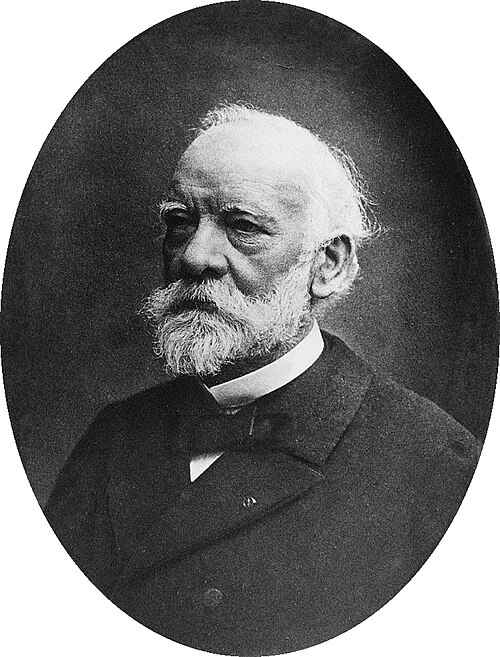
\includegraphics[width=\linewidth]{images/book3/friedel.jpg}
\end{minipage}\hspace{0.02\linewidth}%
\begin{minipage}[t]{0.18\linewidth}
\vspace{0pt}
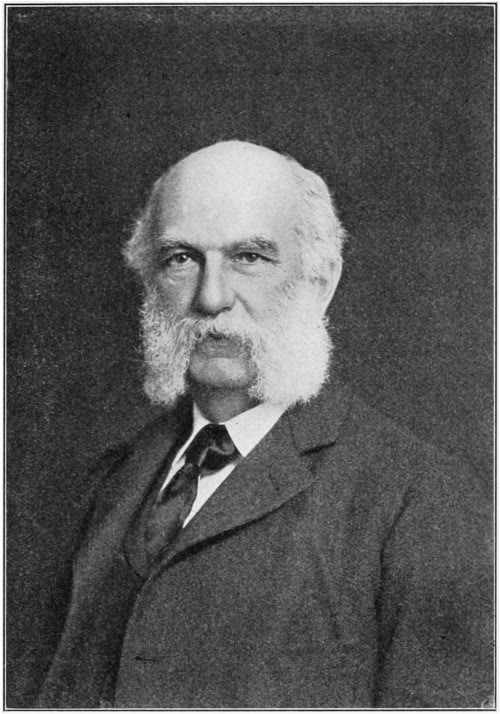
\includegraphics[width=\linewidth]{images/book3/crafts.jpg}
\end{minipage}\hfill
\begin{minipage}[t]{0.58\linewidth}
\vspace{0pt}
1877 में पेरिस में साथ काम करते हुए शार्ल फ़्रीडेल और जेम्स मेसन क्राफ़्ट्स ने पाया कि
ऐलुमिनियम क्लोराइड हैलोऐल्केनों और ऐसिल क्लोराइडों को बेन्ज़ीन से अभिक्रिया कराता है। उनकी
अभिक्रियाएँ \omterm{def:b2:huckel:aromatic}{ऐरोमैटिक} वलयों पर कार्बन समूह जोड़ने का मानक तरीका बन गईं, और उनके द्वारा खोजा गया
लुइस अम्ल उत्प्रेरण इससे बहुत आगे तक पहुँचा। (चित्र: फ़्रीडेल, 1890 का दशक; क्राफ़्ट्स,
\textit{पॉपुलर साइंस मंथली} से, 1900; सार्वजनिक अधिकार-क्षेत्र, विकिमीडिया कॉमन्स।)
\end{minipage}
\end{history}

\begin{safety}{\ghs[5mm]{GHS02}\,\ghs[5mm]{GHS05}\,\ghs[5mm]{GHS06}\,\ghs[5mm]{GHS08}}
बेन्ज़ीन कैंसरजनक है और जहाँ भी संभव हो, उसके स्थान पर टॉलूईन या अन्य \omterm{def:b2:aromatic-substitution:arene}{ऐरीन} प्रयुक्त किए जाते हैं।
सांद्र नाइट्रिक और सल्फ़्यूरिक अम्ल संक्षारक हैं और नाइट्रीकारी मिश्रण प्रबल
ऑक्सीकारक है; उसे ठंडा रखा जाता है और \omterm{def:b2:aromatic-substitution:arene}{ऐरीन} धीरे-धीरे मिलाई जाती है, क्योंकि नाइट्रीकरण \omterm{def:b2:reaction-enthalpy:exothermic}{ऊष्माक्षेपी} होते हैं।
ब्रोमीन अत्यंत विषैली और संक्षारक है; ऐलुमिनियम क्लोराइड जल से प्रचंड अभिक्रिया करता है। नाइट्रोऐरीन
विषैले हैं।
% ledger: ghs:benzene, ghs:toluene, ghs:HNO3, ghs:H2SO4, ghs:Br2, ghs:AlCl3, ghs:nitrotoluene-4
\end{safety}

\section{अभ्यास}

\begin{exercise}[$\star$]\label{exo:b2:aromatic-substitution:1}
नाइट्रिक अम्ल और सल्फ़्यूरिक अम्ल से नाइट्रोनियम आयन का बनना लिखिए।
\end{exercise}

\begin{exercise}[$\star$]\label{exo:b2:aromatic-substitution:2}
टॉलूईन और नाइट्रोबेन्ज़ीन के ब्रोमीनन (\ce{Br2}, \ce{FeBr3}) के मुख्य उत्पाद
दीजिए।
\end{exercise}

\begin{exercise}[$\star$]\label{exo:b2:aromatic-substitution:3}
सक्रियक या निष्क्रियक, ऑर्थो/पैरा या मेटा के रूप में वर्गीकृत कीजिए: \ce{-CH3}, \ce{-OH}, \ce{-Cl},
\ce{-NO2}, \ce{-COCH3}, \ce{-NHCOCH3}।
\end{exercise}

\begin{exercise}[$\star$]\label{exo:b2:aromatic-substitution:4}
एथेनॉयल क्लोराइड और ऐलुमिनियम क्लोराइड के साथ बेन्ज़ीन का उत्पाद दीजिए।
\end{exercise}

\begin{exercise}[$\star\star$]\label{exo:b2:aromatic-substitution:5}
\ce{AlCl3} के साथ बेन्ज़ीन और 1-क्लोरोप्रोपेन मुख्यतः आइसोप्रोपिलबेन्ज़ीन देते हैं। समझाइए, और
प्रोपिलबेन्ज़ीन तक एक दो-चरणीय मार्ग दीजिए।
\end{exercise}

\begin{exercise}[$\star\star$]\label{exo:b2:aromatic-substitution:6}
फ़ीनॉल ब्रोमीन जल को तुरंत, बिना उत्प्रेरक के, रंगहीन कर देता है और
2,4,6-ट्राइब्रोमोफ़ीनॉल देता है। समझाइए।
\end{exercise}

\begin{exercise}[$\star\star$]\label{exo:b2:aromatic-substitution:7}
बेन्ज़ीन से 3-ब्रोमोनाइट्रोबेन्ज़ीन और 4-ब्रोमोनाइट्रोबेन्ज़ीन के संश्लेषण दीजिए।
\end{exercise}

\begin{exercise}[$\star\star$]\label{exo:b2:aromatic-substitution:8}
ऐनिलीन का नाइट्रीकरण ठीक से नहीं होता (ऑक्सीकरण, और मेटा उत्पाद), परंतु ऐसीटैनिलाइड मुख्यतः
4-नाइट्रोऐसीटैनिलाइड देता है। दोनों तथ्यों को समझाइए।
\end{exercise}

\begin{exercise}[$\star\star$]\label{exo:b2:aromatic-substitution:9}
दिखाइए कि सल्फ़ोनिक अम्ल समूह का उपयोग पैरा समावयवी से मुक्त 2-ब्रोमोटॉलूईन बनाने में कैसे किया जा सकता है।
\end{exercise}

\begin{exercise}[$\star\star\star$]\label{exo:b2:aromatic-substitution:10}
4-मेथिलऐनिसोल (4-मेथॉक्सीटॉलूईन) का नाइट्रीकरण कहाँ होता है? दोनों निर्देशक समूहों के आधार पर
समझाइए।
\end{exercise}

\begin{exercise}[$\star\star\star$]\label{exo:b2:aromatic-substitution:11}
2,4,6-ट्राइनाइट्रोटॉलूईन टॉलूईन के तीन क्रमिक नाइट्रीकरणों से बनाया जाता है, हर एक पिछले से कठोर
परिस्थितियों में। समझाइए क्यों।
\end{exercise}

\begin{exercise}[$\star\star\star$]\label{exo:b2:aromatic-substitution:12}
टॉलूईन से 4-नाइट्रोबेन्ज़ोइक अम्ल का, और 3-नाइट्रोबेन्ज़ोइक अम्ल का, एक संश्लेषण प्रस्तावित कीजिए।
\end{exercise}

\section{समस्या: टॉलूईन का नाइट्रीकरण}

\begin{problem}[{सप्ताहांत समस्या --- नाइट्रोनियम आयन और नाइट्रीकरण की क्रियाविधि, सांख्यिकीय
अनुपात की तुलना में टॉलूईन की ऑर्थो, मेटा और पैरा स्थितियाँ, समावयवियों का
पृथक्करण, और एक द्रव्यमान संतुलन}]
\label{pb:b2:aromatic-substitution:1}
आँकड़े: गलनांक: 2-नाइट्रोटॉलूईन \qty{-10}{\degreeCelsius}, 3-नाइट्रोटॉलूईन
\qty{16}{\degreeCelsius}, 4-नाइट्रोटॉलूईन \qty{52}{\degreeCelsius}। एक प्रयोग के लिए अभ्यास के आँकड़े:
टॉलूईन के \qty{100}{g}, \omterm{def:b2:continuous-reactors:conversion}{रूपांतरण} 90~\%, समावयवी वितरण 58~\% ऑर्थो, 4~\% मेटा,
38~\% पैरा। मोलर द्रव्यमान (\unit{g/mol}): C 12.011, H 1.008, N 14.007, O 15.999।
% ledger: mp:2-nitrotoluene, mp:3-nitrotoluene, mp:4-nitrotoluene, aw:C, aw:H, aw:N, aw:O

\medskip
\noindent\textbf{भाग I --- इलेक्ट्रॉनरागी और क्रियाविधि।}
\begin{enumerate}
  \item नाइट्रोनियम आयन का बनना लिखिए।
  \item इसकी लुइस संरचना खींचिए और इसकी आकृति बताइए।
  \item मेथिल के पैरा स्थान पर टॉलूईन पर \ce{NO2+} का आक्रमण लिखिए।
  \item पैरा \omterm{def:b2:aromatic-substitution:seAr}{व्हीलैंड मध्यवर्ती} की तीन अनुनादी संरचनाएँ खींचिए।
  \item कौन-सा चरण दर-निर्धारक है?
  \item दूसरे चरण में प्रोटॉन को कौन हटाता है?
\end{enumerate}

\medskip
\noindent\textbf{भाग II --- तीनों स्थितियाँ।}
\begin{enumerate}[resume]
  \item टॉलूईन की कितनी ऑर्थो, मेटा और पैरा स्थितियाँ हैं?
  \item यादृच्छिक आक्रमण कौन-सा अनुपात देता?
  \item मेटा \omterm{def:b2:aromatic-substitution:seAr}{व्हीलैंड मध्यवर्ती} खींचिए और समझाइए कि वह सबसे कम स्थायीकृत क्यों है।
  \item मेथिल समूह ऑर्थो और पैरा मध्यवर्तियों को कैसे स्थायी करता है?
  \item प्रेक्षित अनुपात की सांख्यिकीय अनुपात से तुलना कीजिए: कौन-सी स्थितियाँ अनुकूल हैं?
  \item ऑर्थो (ऑर्थो प्रतिशत का आधा) और पैरा पर प्रति स्थिति लब्धि की तुलना कीजिए।
        अंतर का एक कारण सुझाइए।
  \item क्या टॉलूईन का नाइट्रीकरण बेन्ज़ीन से तेज़ होता है या धीमा?
\end{enumerate}

\medskip
\noindent\textbf{भाग III --- पृथक्करण।}
\begin{enumerate}[resume]
  \item कमरे के ताप पर कौन-सा समावयवी ठोस है?
  \item सुझाइए कि ठंडा करके उसे मिश्रण से कैसे पृथक किया जाए।
  \item सममिति उच्च गलनांक के अनुकूल क्यों होती है?
  \item बाद में ऑर्थो और मेटा समावयवियों को कैसे पृथक किया जा सकता है?
  \item इन समावयवियों को साधारण आसवन से पृथक करना कठिन क्यों है?
\end{enumerate}

\medskip
\noindent\textbf{भाग IV --- द्रव्यमान संतुलन।}
\begin{enumerate}[resume]
  \item टॉलूईन और नाइट्रोटॉलूईन का मोलर द्रव्यमान परिकलित कीजिए।
  \item टॉलूईन की मात्रा और बने नाइट्रोटॉलूईन की मात्रा परिकलित कीजिए।
  \item तीनों समावयवियों के द्रव्यमान परिकलित कीजिए।
  \item ठंडा करके और अम्ल का आधिक्य प्रयुक्त न करके कौन-सी आगे की अभिक्रिया से बचना चाहिए?
  \item पैरा समावयवी से आप 4-नाइट्रोबेन्ज़ोइक अम्ल कैसे बनाएँगे?
  \item इस प्रयोग में टॉलूईन के \qty{100}{g} से प्राप्त 4-नाइट्रोटॉलूईन का द्रव्यमान बताइए।
\end{enumerate}
\end{problem}
